\documentclass{book}
\author{Michiel Baptist}
\title{On The Basics Of ... For Dummies}


\usepackage{amsthm}
\usepackage{tikz}
\usepackage{amsmath}
\usepackage{amssymb}
\usepackage{bbm}
\usepackage{algorithm}
\usepackage{algorithmic}
\usepackage{graphicx}
\usepackage{amsfonts}
\usepackage{hyperref}

\newcommand{\this}{NONE}
\newcommand{\base}{chapters}
\newcommand{\figDir}{\base/\this/fig}

\newcommand{\norm}[1]{\left\lVert#1\right\rVert}
\newcommand{\der}[1]{\frac{d}{d #1}}
\newcommand{\ID}{\mathbbm{1}}
\newcommand{\Real}{\mathbb{R}}
\newcommand{\Compl}{\mathbb{C}}
\newcommand{\Det}[1]{
	\begin{vmatrix}
		#1\\
	\end{vmatrix}
}
\newcommand{\hVec}[1]{
	\begin{pmatrix}
		#1
	\end{pmatrix}
}

\theoremstyle{plain}
\newtheorem{thm}{Theorem}[chapter] % reset theorem numbering for each chapter

\theoremstyle{definition}
\newtheorem{defn}{Definition} % definition numbers are dependent on theorem numbers
\newtheorem{exmp}{Example} % same for example numbers


\begin{document}
	\maketitle
	Introduction goes here:
		- Book by me for me
		- Book of derivations, theory, usefullness
		- Fill in as I go
		- ...
	\tableofcontents
	\chapter*{Definitions and notation}

In this section I present an overview of the mathematical 
notation I employ and some of the more common definitions.
Each definition comes with a little intuition, or at least
a view into my own way of thinking about the respective 
definitions. Whenever a definition is mentioned in the text,
this chapter is referred to.

\section*{Notation}

\section*{Commonly used definitions}

\subsection*{1. Norms}
Humans usually like to compare things to each other.
Which apple is riper, juicier and generally better looking?
Do I procrastinate, do I try to be productive? Often one or 
several criteria are compared. Color of the apple, size of 
the apple, and so on. In mathematics, humans have implemented 
a very similar notion upon objects such as vectors and matrices. 
This notion is called a \textit{norm}. It's definition is 
rather simple, but elegant:

\begin{defn} [Mathematical norm]
Given a vector space $V$ in over a field in $\Real$ or 
$\Compl$. A norm $\norm{.}$ is a function 
$\norm{.}:V \mapsto \Real$ such that $\forall v, u \in V$:

\begin{enumerate}
\item $\norm{v} \geq 0$
\item $\norm{v + u} \leq \norm{v} + \norm{u}$
\item $\norm{av} = |a|\norm{v}$ $\forall a \in \Real$
\item $\norm{v} = 0 \Leftrightarrow v = 0$
\end{enumerate}

Condition 2 is called the triangle inequality. Note that
the definition of norm might allow many definitions. 
Not only the norms such as the euclidean norm (p-norm) for example.
\end{defn}
\begin{defn}[The $\mathcal{L}^p$ norm or the p-norm]
The $\mathcal{L}^p$ norm or p-norm $\norm{.}_p$ is 
defined over $n$ dimensional vector spaces. It is given by:
\begin{equation}
\norm{x}_p = \bigg( \sum_{i=1}^{n} |x_i|^p \bigg)^\frac{1}{p}
\end{equation}
\end{defn}
These types of norms are most commonly used in 
statistics and mathematics. The \textit{Euclidean} norm is
simply the $\mathcal{L}^2$ norm. The $\mathcal{L}^1$ norm is
usually referred to as the taxicab norm or the 
Manhattan norm. To see why consider taking a taxi to point
$(2,3)$ in the plane and the driver is only allowed to drive
horizontally and vertically. The taxicab norm is then
simply the total amount of driven distance.
\\\\
So far we described norms in terms of $1 \times m$ 
dimensional vectors. The concept of a norm for matrices is 
somewhat less intuitive. However, some matrix norms are.
Take for example the Frobenius norm, it is the natural extension
of the $\mathcal{L}^2$ norm for vectors.
\begin{defn}[Frobenius norm]
The frobenius norm is defined over $m\times n$ 
matrices $X \in \Real^{m \times n}$. It is the 
natural extension of the 2-norm for vectors. It is defined as: 
\begin{equation}
\label{eq:def_frobenius}
\begin{split}
\norm{X}_F &= \sqrt{\sum_{i=1}^{m}\sum_{j=1}^{n}|x_{ij}|^2}\\
&= \sqrt{trace(X^TX)} \\
\end{split}
\end{equation}
\end{defn}
To see why the second line in equation \ref{eq:def_frobenius}
holds, let's write out $trace(X^TX)$.
\begin{equation}
\begin{split}
trace(X^TX) &= trace
\begin{pmatrix}
\horzbar & x_1 & \horzbar\\
 & \vdots & \\
\horzbar & x_n & \horzbar\\
\end{pmatrix}
\begin{pmatrix}
\vertbar & & \vertbar\\
 x_1 & \hdots & x_n \\
\vertbar & & \vertbar\\
\end{pmatrix}\\
&= trace
\begin{pmatrix}
x_1^Tx_1 & & &\\
& x_2^Tx_2 & &\\
& & & \ddots &\\
& & & & x_n^Tx_n\\
\end{pmatrix}\\
&= \sum_{i = 1}^{n} x_i^Tx_i\\
&= \sum_{i = 1}^{n} \bigg( \sum_{j=1}^{m} x_{ij}^2 \bigg)
\end{split}
\end{equation}

\section*{Matrix properties}
\begin{defn}[Idempotent matrix]
A matrix $A$ is idempotent iff $AA = A$.
\end{defn}

\begin{prop}
Let $X \in \Real^{m \times n}$ then
\begin{equation}
XX^T = \sum_{i=1}^{n}x_ix_i^T
\end{equation}
\end{prop}

\begin{proof}
Depending on your viewpoint of matrix multiplication this property
might seem trivial to prove. However, here is one way. Let's begin 
from the left side of the equation:
\begin{equation}
\begin{split}
XX^T &=
\begin{pmatrix}
\horzbar & x_1 & \horzbar \\
& \hdots & \\
\horzbar & x_m & \horzbar \\
\end{pmatrix}
\begin{pmatrix}
\vertbar & & \vertbar \\
x_1 & & x_m \\
\vertbar & & \vertbar \\
\end{pmatrix}\\
&= \begin{pmatrix}
\norm{x_1}^2 & x_{1} x_{2}^T& \\
x_2 x_1^T & \norm{x_2}^2 &  & \\
& & \ddots & \\
& & & \norm{x_m}^2\\
\end{pmatrix}\\
&= \begin{pmatrix}
\sum_{j=1}^{n}x_{1j}^2 & \sum_{j=1}^{n} x_{1j}x_{2j} & \\
\sum_{j=1}^{n} x_{1j}x_{2j} & \sum_{j=1}^{n}x_{2j}^2  &  & \\
& & \ddots & \\
& & & \sum_{j=1}^{n}x_{mj}^2 \\
\end{pmatrix}\\
&= \sum_{j=1}^{n}
\begin{pmatrix}
x_{1j}^2 & x_{1j}x_{2j} & \\
x_{1j}x_{2j} & x_{2j}^2  &  & \\
& & \ddots & \\
& & & x_{nj}^2 \\
\end{pmatrix}\\
&= \sum_{j=1}^{n} x_jx_j^T
\end{split}
\end{equation}
\end{proof}
\section*{Matrix derivatives}

\begin{prop}
Given vector $b \in \Real^m$ and symmetric matrix 
$X \ in \Real^{m \times m}$ then it holds that:
\begin{equation}
\nabla_b b^TXb = 2Xb
\end{equation}
\end{prop}
\begin{proof}
Let's write out the $b^tXb$:
\begin{equation}
\begin{split}
b^T X b &= \sum_{i=1}^{m} b_i (Xb)_i\\
&= \sum_{i=1}^{m} b_i \big( \sum_{j=1}^{m} x_{ij}b_j\big)\\
&= \sum_{i=1}^{m}\sum_{j=1}^{m} b_i b_j x_{ij}\\
\end{split}
\end{equation}
Finding the partial derivative for a given $b_k$ is then
straight forward:
\begin{equation}
\begin{split}
\pd{x_k}
	\sum_{i=1}^{m}\sum_{j=1}^{m} b_i b_j x_{ij} 
	&= 
	  2b_kx_{kk} 
	+ \sum_{\substack{j=1\\ j\neq k}}^{m} b_jx_{kj} 
	+ \sum_{\substack{j=1\\ j\neq k}}^{m} b_jx_{jk} 
\\&=
	2\sum_{j=1}^{m} b_jx_{kj}
\\&=
	2x_kb_j
\end{split}
\end{equation}
The gradient is defined as:
\begin{equation}
\nabla_x f(x)= 
\begin{pmatrix}
\frac{\partial}{\partial x_1} f(x)\\
\vdots \\
\frac{\partial}{\partial x_m} f(x)\\
\end{pmatrix}
=2
\begin{pmatrix}
x_1 b\\
\vdots \\
x_m b
\end{pmatrix}
=
2Xb
\end{equation}
\end{proof}

\begin{prop}
$\nabla_x \norm{x}^2 = 2x$
\end{prop}
\begin{proof}
We find the partial derivative for $x_i$:
\begin{equation}
\begin{split}
\frac{\partial}{\partial x_i} \norm{x}^2 &= 
	\frac{\partial}{\partial x_i} x^Tx \\
&= \frac{\partial}{\partial x_i} \sum_{j=1}^{m} x_j^2 \\
&= 2x_i
\end{split}
\end{equation}
The gradient is defined as:
\begin{equation}
\nabla_x f(x)= 
\begin{pmatrix}
\frac{\partial}{\partial x_1} f(x)\\
\vdots \\
\frac{\partial}{\partial x_m} f(x)\\
\end{pmatrix}
=2
\begin{pmatrix}
x_1\\
\vdots \\
x_m
\end{pmatrix}
\end{equation}
\end{proof}

\begin{prop}
$\nabla_x \norm{Ax}^2 = 2A^TAx = 2(Ax)^TA$ 
\end{prop}

\begin{proof}
\label{sec:gradient_squared_norm}
This proof is long and winded. However, it gives you intuition.
In the following, $a_i$ is the $i$'th row of $A$. $a_{.k}$
is by extension the $k$'th column of $A$.
Let's begin by taking a partial derivative for $x_i$:
\begin{equation}
\begin{split}
\pd{x_k} \norm{Ax}^2 
&= \pd{x_k} \Bigg\langle 
\begin{pmatrix}
a_1x \\
\vdots \\
a_mx
\end{pmatrix},
\begin{pmatrix}
a_1x \\
\vdots \\
a_mx \\
\end{pmatrix} \Bigg\rangle \\
&= \pd{x_k}\sum_{i=1}^{m} (a_ix)^2 \\
&= \pd{x_k}\sum_{i=1}^{m} \Big(\sum_{j=1}^{m} a_{ij}x_j\Big)^2 \\
&= 2\sum_{i=1}^{m}\Big(\sum_{j=1}^{m} a_{ij}x_j \Big) \pd{x_k} 
		\Big(\sum_{j=1}^{m} a_{ij}x_j \Big)\\
&= 2\sum_{i=1}^{m}\Big(\sum_{j=1}^{m} a_{ij}x_j \Big) a_{ik} \\
&= 2\sum_{i=1}^{m}(a_ix)a_{ik}
\end{split}
\end{equation}
In the above equation $(a_ix)$ is the $i$'th element of $Ax$.
Since $i$ is going from $1 \rightarrow m$ we see in the last line
that we are multiplying $Ax$ by the $k$'th column of $A$.
We rewrite as follows:
\begin{equation}
\pd{x_i} \norm{Ax}^2 = 2(Ax)^TA_{.k}
\end{equation}
The gradient is defined as:
\begin{equation}
\begin{split}
\nabla_x f(x)&= 
\begin{pmatrix}
\frac{\partial}{\partial x_1} f(x)\\
\vdots \\
\frac{\partial}{\partial x_m} f(x)\\
\end{pmatrix}
=2
\begin{pmatrix}
(Ax)^TA_{.1}\\
\vdots \\
(Ax)^TA_{.m} \\
\end{pmatrix} \\
&= 2(Ax)^T\begin{pmatrix}
A_{.1} &
\hdots &
A_{.m}
\end{pmatrix} \\
&= 2 (Ax)^T A
\end{split}
\end{equation}
\end{proof}
	\renewcommand{\this}{PCA}

\chapter{Principle Component Analysis (PCA)}
\section{Matrix factorization as a tool}
The core concept of principle component analysis is 
making use of matrix factorization techniques. These 
techniques, as the name implies, decompose a matrix 
of interest $X \in \Real^{m \times n}$ into several 
matrices such that their product equals $X$. For 
example, an approximation of the data matrix $X$ 
could be given by the product of 
$A \in \Real^{m \times k}$ and $B \in \Real^{k \times n}$:
\\
\begin{figure}[h!]
	\centering	
	\begin{tikzpicture}
	\draw (0,0) node[shape=rectangle, 
					 draw=black, 
					 minimum width = 40, 
					 minimum height = 30](x){$X$};
	\draw node[below of = x] (times) {$m \times n$};
	\draw node[right of = x, xshift = 2ex] (apr){$\approx$};
			
	\draw node[right of = apr, 
			   shape=rectangle, 
			   draw=black, 
			   minimum width = 20, 
			   minimum height = 30](A){$A$};
			   
	\draw node[below of = A] (times) {$m \times k$};
			
	\draw node[right of = A, 
			   shape=rectangle, 
			   draw=black, 
			   minimum width = 40, 
			   minimum height = 20, 
			   xshift = 2ex](B){$B$};
	\draw node[below of = B] (times) {$k \times n$};
	\end{tikzpicture}
	\label{approx}
	\caption{Example of factorization.}
\end{figure}\\
A whole range of practical problems can be written
as a matrix factorization problems. Often we can 
gain a lot of insights based on decompositions.
\\\\
In the previous example, the matrix $X$ was a $m \times n$ matrix. 
It was decomposed into $m \times k$ and $k \times n$ matrices. 
Naturally, $A$ and $B$ share a dimension such that their product
is defined. In matrix factorization problems this is almost always
the case. This $k$ can be chosen differently based on the problem 
you are dealing with. For example, if one wants to decompose a 
matrix without losing any information at all, one chooses 
$k = \min(m, n)$. It is not always desirable to decompose a 
given matrix, without losing information. In most cases one is
interested in smaller $k$ values. Be it for reducing dimension, 
easier understanding of the decomposition, memory and time 
considerations.

\section{Frobenius norm as a closeness metric}
\label{sec:frobenius}
When using a $k$ value smaller than $\min(m, n)$, we lose 
information when decomposing matrix $X \Real^{m\times n}$.
The decomposition then becomes an approximation $X \approx AB$
As we don't want to lose too much information, we need a 
measure of how \textit{close} two matrices are. 
One of the ways we can measure this is using the frobenius norm:
\begin{equation}
	d(A, B) = \norm{A - B}_F
\end{equation}
Assume again, we wish to find a matrix decomposition of $X$ where 
$k$ is small, so we lose information, the decomposition is
an approximation. We would then measure how good this approximation
is using the frobenius norm:
\begin{equation}
	d(X,AB) = \norm{X - AB}_F
\end{equation}
Transforming this into a minimization objective:
\begin{equation}
	\underset{A,B}{\min}\norm{X - AB}_F
\end{equation}
	
\section{PCA as dimension reduction}
PCA is primarily a technique to \textit{reduce the dimension} of 
a given data set $X$. Assume there are $n$ data points
of dimension $m$, i.e.
$\mathcal{X} = \{x_i| x_i \in \Real^m, i \in \{1\dots n\}\}$.
Conveniently, this can be encapsulated as a matrix 
$X \in \Real^{n \times n}$. We can then decompose the 
matrix as before into $A \in \Real^{m \times k}$ and 
$B \in \Real^{k \times n}$. Assume now that $k$ is 
significantly smaller $\min(m,n)$. Instead of having 
$\mathcal{O}(mn)$ values we now only have $\mathcal{O}(k(m+n))$
values. For a large $m$ this is significant. The above
was an example of dimension reduction. PCA is an example of 
such a dimension reduction techniques. Even more, it is 
one of the most used techniques out there for reducing dimension.

\begin{exmp}
As an example we could look at an approximation of a face using PCA.
\begin{figure}[h!]
	\centering
	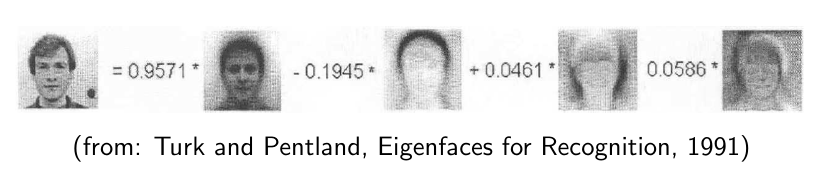
\includegraphics[scale=0.5]{\figDir/face_ex.PNG}
\end{figure}\\
The dimension of the original data points is the 
exact amount of pixels in the image. Perhaps the amount
of pixels is unmanageable. In this example, the faces were
are reconstructed using $k=4$ images. Thus, instead of 
considering each data point as a collection of pixels,
we reduced the dimension of the data by considering each data 
point as a combination of $4$ base images. We have reduced 
the dimension of the data to $4$. Of course, in order 
to re-construct the original images, the $4$ base images 
are required.
\end{exmp}

\section{Reducing data to a single value}
In order to see what PCA does exactly, we will first
consider what would happen if we reduced the $m$ dimensional
data to a single value. Hopefully, this value will contain 
the most information as possible. In essence we are looking 
at what would happen as $k = 1$. In order to reduce each data 
point to a single value, many approaches exist. Take for example
the approach where we simply take the euclidean norm of each point.
In this case, we capture some information but we lose a lot
of information. To see why consider $(0, 1)$ and $(1, 0)$.
They are perpendicular, yet $\norm{(0,1)} = \norm{(1,0)}$.
\\\\
There are better ways. We could for instance reduce the points
by projecting them onto a single line. This is actually the first
and only step in PCA. By iterating this exact step we obtain
the PCA decomposition. We start by projecting onto a single line.

\subsection{Projecting a single data point onto a fixed line}
Before we project onto it, we need to define exactly what 
is meant with a line in the $\Real^m$ space.
One way to define a line is as follows:

\begin{defn}
\begin{equation}
a + \Real b \equiv \{x \in \Real^m | 
\exists z \in \Real \text{ s.t. } x = a + zb\}
\end{equation}
Here, $a$ is sometimes referred to as the offset or intercept
and $b$ is sometimes referred to as the direction of the line.
\end{defn}
			
\begin{figure}[h!]
	\centering
	\begin{tikzpicture}[scale = 0.5]
	\draw[->] (-1,0) -- (5,0);
	\draw[->] (0,-1) -- (0,5);
	\draw[->, red, thick] (0,0) -- node[xshift = 1.5ex](lab){a}(1,2);
	\draw[->, blue, thick] (1,2) -- node[xshift = 1.5ex](lab){b}(2,1);
	\draw[blue, dashed] (-1,4) -- node[xshift = 1.5ex](lab){b}(4,-1);
	\end{tikzpicture}
	\label{fig:line}
	\caption{Visual of a line}
\end{figure}

Figure \ref{fig:line} gives an intuitive idea of 
what a line in $\Real^2$ looks like. Often we want the 
direction to have unit length. Mathematically this means: 
$\norm{b}_2 = 1$.
\\\\
Say we want to project a point $x$ onto a single line. There are
infinite ways to do this. However, if one wants to keep
as much of the information contained in the original 
point, we need to define an objective function.
Ideally, this objective function defines how distant the
projected point and the original point are. This concept 
should sound familiar. Just as in section \ref{sec:frobenius},
we defined the Frobenius norm as a metric to measure how
distance two matrices are. As the Frobenius norm is the 
natural extension of the $\mathcal{L}^2$ norm. Let's use 
the $\mathcal{L}^2$ norm to measure distance between
two points.
\\\\
We know that the projected point is somewhere on the line
we are projecting to. Let's call this point $a + bz$, we know
our line is fixed. This means $a$ and $b$ are fixed. Thus, the projected
point is completely defined by $z$. The squared euclidean
distance between the two points is then defined as:
\begin{equation}
\label{eq:eucl_proj}
\underset{z\in\Real}{\text{arg min}} \norm{a + bz - x}^2
\end{equation}

Figure \ref{fig:sq} shows an intuitive picture of 
the \textbf{non squared} euclidean distance. There are
\begin{figure}[h!]
	\centering
	\begin{tikzpicture}[scale = 0.5]
	\draw[->] (-1,0) -- (5,0);
	\draw[->] (0,-1) -- (0,5);
					
	\draw (4,2) circle (0.1cm);
					
	\draw[->, red, thick] (0,0) -- node[xshift = 1.5ex](lab){a}(1,2);
	\draw[->, blue, thick] (1,2) -- node[xshift = 1.5ex](lab){b}(2,1);
	\draw[blue, dashed] (-1,4) -- node[xshift = 1.5ex](lab){b}(4,-1);
					
	\draw[dashed] (4,2) -- (2.5,0.45);
	\draw[dashed] (4,2) -- node[yshift = 1ex] {$z_1$} (-0.5,3.5);
	\draw[dashed] (4,2) -- node[xshift = 1ex] {$z_3$}(4,-1);
	\end{tikzpicture}
	\caption{Visual of distance to a line for varying $z$ values}
	\label{fig:sq}
\end{figure}\\

It is clear to see that using the squared euclidean distance 
that we reach the optimal point on the line by projecting the
original point orthagonally onto the line. 
Mathematically we can find this by deriving the squared
euclidean distance in equation \ref{eq:eucl_proj} for $z$.
\begin{equation}
\label{eq:sol_z}
\begin{split}
\der{z}\norm{a + bz - x}^2 &= 2(a +bz - x)^T b = 0 \\
&=(a-x)^T b + \underbrace{b^Tb }_{\norm{b}^2 = 1}z = 0\\
z &=-(a-x)^Tb
\end{split}
\end{equation}
This confirms our belief that the orthogonal projection 
does indeed minimize the distance between the original 
data point and the projected data point. We see this 
since we are projecting onto the $b$ direction.
\\\\
To understand 
exactly what's happening we can have a look at figure
\ref{fig:proj}. Here, the green arrow ($x-a$) is being 
projected onto $b$ to find the optimal $z$.
\begin{figure}[h!]
	\centering
	\begin{tikzpicture}[scale = 0.5]
	\coordinate[](origin) at (0,0) ;
	\coordinate[](a) at (1,2) ;
	\coordinate[](b) at (2,1) ;
	\coordinate[](x) at (4,2) ;
	
	\draw[->] (-1,0) -- (5,0);
	\draw[->] (0,-1) -- (0,5);
	
	\draw (x) circle (0.1cm);
	
	\draw[->, red, thick] (origin) -- node[xshift = 1.5ex](lab){a}(a);
	\draw[->, blue, thick] (a) -- node[xshift = 1.5ex](lab){b}(b);
	\draw[blue, dashed] (-1,4) -- node[xshift = 1.5ex](lab){b}(4,-1);
	
	\draw[thick, green, ->] (a)--(x);
	\draw[dashed] (4,2) -- (2.5,0.45);
	\end{tikzpicture}
	\caption{Visual of optimal $z$ value as a 
	projection of $(x-a)$ onto the direction.}
	\label{fig:proj}
\end{figure}
Now that we found the $z$ value that minimizes the 
loss (the projection onto the $b$ direction), let's look 
at what this means mathematically:
\begin{equation}
\label{eq:x_prime}
x' = a + (x-a)^Tbb
\end{equation} 
To better visualize this result, we can have a look at
figure \ref{fig:recon}.
\begin{figure}[h!]
	\centering
	\begin{tikzpicture}[scale = 0.5]
	\coordinate[](origin) at (0,0) ;
	\coordinate[](a) at (1,2) ;
	\coordinate[](b) at (2,1) ;
	\coordinate[](x) at (4,2) ;
	
	\draw[->] (-1,0) -- (5,0);
	\draw[->] (0,-1) -- (0,5);
	
	\draw (x) circle (0.1cm);
	
	\draw[->, red, thick] (origin) -- node[xshift = 1.5ex](lab){a}(a);
	\draw[->, blue, thick] (a) -- node[xshift = 1.5ex](lab){b}(b);
	\draw[blue, dashed] (-1,4) -- node[xshift = 1.5ex](lab){b}(4,-1);
	
	\draw[thick, green, ->] (a)--node[yshift = 1ex]{$x-a$}(x);
	\draw[dashed] (4,2) -- (2.5,0.45);
	\draw[black, ->, thick] (origin) 
		--node[xshift = -6ex] {$(x-a)^Tb$} (1.3,-1.3);
	\end{tikzpicture}
	\begin{tikzpicture}[scale = 0.5]
	\coordinate[](origin) at (0,0) ;
	\coordinate[](a) at (1,2) ;
	\coordinate[](b) at (2,1) ;
	\coordinate[](x) at (4,2) ;
	
	\draw[->] (-1,0) -- (5,0);
	\draw[->] (0,-1) -- (0,5);
	
	\draw (x) circle (0.1cm);
	
	\draw[->, red, thick] (origin) -- node[xshift = 1.5ex](lab){a}(a);
	\draw[->, blue, thick] (a) -- node[xshift = 1.5ex](lab){b}(b);
	\draw[blue, dashed] (-1,4) -- node[xshift = 1.5ex](lab){b}(4,-1);
	\draw[black, ->, thick] (origin) 
			--node[xshift = -6ex] {$(x-a)^Tb$} (1.3,-1.3);
	
	\draw[dashed, ->, bend right = 45, purple]
		(1,-1)to node[xshift = 1ex]{$+a$}(2.2,0.8);
			
	\end{tikzpicture}
	\caption{Visual of optimal $z$ value 
			plugged back in to find the optimal point again.}
	\label{fig:recon}
\end{figure}
Mathematically, the story being told by equation \ref{eq:x_prime} is
quite logical. We can see 4 steps:
\begin{enumerate}
	\item Remove the intercept from $x$: $x-a$
	\item Project orthagonally onto $b$: $(x-a)^Tb$
	\item Multiply in the $b$ direction: $(x-a)^Tbb$
	\item Add back the intercept: $(x-a)^Tbb + a$
\end{enumerate}
So by minimizing the euclidean distance from a point
to a line we find the orthogonal projection. This will
be used extensively in the next few sections.

\subsection{Optimal line through multiple data points}
We've seen how to optimally project a single data 
point to a fixed line, minimizing euclidean distance.
We now look at what happens when we have more than a single
data point. Additionally, we don't consider the line $a + b\Real$
to be fixed. Instead, we turn the exercise upside down. We
want to answer the question: \textit{what would be the optimal
line through our data points, such that when we project all points
orthagonally, we keep as much information as possible?} In line
with the previous sections, we measure \textit{information} loss
using the euclidean distance.
\\\\
Mathematically, we wish to answer the following.
Consider $n$ data points $\{x_1,...,x_n\}$ where $x_i \in \Real^m$.
How do we find the optimal line considering the mean 
squared euclidean loss:
\begin{equation}
\label{eq:loss_ab}
L(a,b) = \frac{1}{n}\sum_{i=1}^{n}\norm{a + bz_i - x_i}
\end{equation}
Additionally we will consider $\norm{b} = 1$, $b$ is a unit 
length vector. This property will become important.
From previous the previous section, we already know that the optimal
$z_i$ for each individual data point in known to be 
$z_i = (x_i-a)^Tbb$. Due to the fact that one projection
of a data point does not interfere with another, we can simply
replace $z_i$ in equation \ref{eq:loss_ab}.
\\\\
Minimizing over $a$ and $b$ and using previous 
results of equation (\ref{eq:sol_z}) we find:

\begin{equation}
\label{eq:loss}
\begin{split}
\argmin_{a, b}\frac{1}{n}\sum_{i=1}^{n}\norm{a + bz_i - x_i}^2 &=
\argmin_{a, b}\frac{1}{n}\sum_{i=1}^{n}\norm{a + b(x_i - a)^Tb - x_i}^2
\\
&= \argmin_{a, b}\frac{1}{n}\sum_{i=1}^{n}
		\norm{bb^T(x_i - a) + (a - x_i)}^2 \\
&= \argmin_{a, b}\frac{1}{n}\sum_{i=1}^{n}
		\norm{bb^T(x_i - a) - (x_i - a)}^2 \\
&= \argmin_{a, b}\frac{1}{n}\sum_{i=1}^{n}
		\norm{(bb^T - \ID_{m})(x_i - a)}^2 \\
\end{split}
\end{equation}
Note that the $\norm{\cdot}$ operation is an even 
function so \ref{eq:loss} can be written equivalently
as (we can change the sign in the brackets 
$\norm{-a} = \norm{a}$):
\begin{equation}
\argmin_{a, b}\frac{1}{n}\sum_{i=1}^{n}\norm{(\ID - bb^T)(x_i - a)}^2 \\
\end{equation}
Now what exactly does the $(\ID_m - bb^T)$ transformation mean?
Transforming a vector $v$ out we obtain:
\begin{equation}
(\ID_m - bb^T)v = v - b(b^Tv)
\end{equation}
Reminding ourselves that $b$ is a unit vector, we can see it
is exactly the vector we obtain when taking the difference
between an original vector $v$ and the projection of the vector
$b(b^Tv)$. Unsurprisingly of course, as that is exactly what we 
started with.
\\\\
A nice thing about $(\ID - bb^T)$ is that it is idempotent.
We can show that this is clearly the case:
\begin{equation}
\label{eq:idempot}
\begin{split}
	(\ID -bb^T)(\ID - bb^t) &= \ID\ID - 2bb^T 
			+ b\underbrace{b^Tb}_{b^Tb = \norm{b}}b^T\\
&= \ID - bb^T\\
\end{split}
\end{equation}\\

\subsection{Optimal value for $a$}
Now let's get back to finding the optimal line for given data. 
The first order optimality condition states that the gradient
with respect to $a$ and $b$ should vanish when optimal.
Taking the gradient with respect to $a$ 
of equation \ref{eq:loss} we find the following:
\begin{equation}
\label{eq:grad_Lin_loss_1}
\begin{split}
\nabla_a L(a,b) &=  \frac{1}{n}\sum_{i=1}^{n}
	\nabla_a\norm{(\ID - bb^T)(x_i - a)}^2 \\
&= \frac{-2}{n}\sum_{i=1}^{n}
	(\ID - bb^T)^T(\ID - bb^T)(x_i - a) \\
&= \frac{-2}{n}(\ID - bb^T)^T
	(\ID - bb^T)\sum_{i=1}^{n}(x_i - a) \\
\end{split}
\end{equation}
In the second line we used the fact that $\nabla_x \norm{Ax}^2 = 2AxA^T$,
which was proven in the definitions section.
We now know that since $(\ID - bb^T)$ is clearly symmetric 
($A^T = A$) and we know that the matrix is idempotent from 
(\ref{eq:idempot}), thus we can write 
(\ref{eq:grad_Lin_loss_1}) follows:
\begin{equation}
\label{eq:grad_Lin_loss_2}
\begin{split}					
	\nabla_a L(a,b) = (\ID - bb^T)\sum_{i=1}^{n}(x_i - a) &= 0\\
	(\ID - bb^T)\sum_{i=1}^{n}(x_i) &= (\ID - bb^T)\sum_{i=1}^{n}(a)\\
	(\ID - bb^T)\frac{1}{n}\sum_{i=1}^{n}(x_i) &= (\ID - bb^T)a\\
\end{split}
\end{equation}
From (\ref{eq:grad_Lin_loss_2}) we can see that the 
optimality condition is met when $a = \frac{1}{n}\sum_{i=1}^{n}x_i$.
This means that the optimal line will always pass through 
the average of all the data points. Figure \ref{fig:avg} 
shows this visually:\\
\begin{figure}[h!]
	\centering				
	\begin{tikzpicture}[scale=0.8]
	\coordinate[](origin) at (0,0) ;
	\coordinate[](x1) at (4,3) ;
	\coordinate[](x2) at (1,2.5) ;
	\coordinate[](x3) at (2,0.5);
	\coordinate[blue](av) at (2.3333333, 2);
	
	\draw (x1) circle (0.1);
	\draw (x2) circle (0.1);
	\draw (x3) circle (0.1);
	\draw[blue, thick, fill = blue] (av) 
			circle (0.05) node[xshift = 2ex]{$\bar{x}$};
	
	\draw[dashed, red] (origin) -- (4.666,4) node[]{$l_1$};
	\draw[dashed, red] (-1,2) -- (5, 2) node[]{$l_2$};
	\draw[dashed, red] (0,4.3333) -- (5,-0.66666) node[]{$l_3$};
	
	\draw[dotted] (av)--(x1) node[xshift = 2ex]{$x_1$};
	\draw[dotted] (av)--(x2) node[xshift = -2ex]{$x_2$};
	\draw[dotted] (av)--(x3) node[xshift = -2ex]{$x_3$};
	
	\draw[->] (-1,0) -- (5,0);
	\draw[->] (0,-1) -- (0,5);
	\end{tikzpicture}
	\caption{Visualisation of lines going 
		through average of data points $x_i$.}
\label{fig:avg}
\end{figure}\\
Figure \ref{fig:avg} shows us visually something quite
interesting, since we know that the optimal line passes 
through the average $\bar{x}$ we could try to make the 
origin itself the average. We could achieve this by 
subtracting the average from every data point as shown 
in figure \ref{fig:subavg}. This step is very often done
as a pre-processing step. It makes derivations easier 
analytically. When "data is centered", this simply means 
that the empirical mean $\frac{1}{n}\sum_{i=1}^{n}x_i$ 
has already been subtracted and that the new mean is the origin.
			
\begin{figure}[h!]
	\centering				
	\begin{tikzpicture}[scale=0.8]
	\coordinate[](origin) at (0,0) ;
	\coordinate[](x1) at (4,3) ;
	\coordinate[](x2) at (1,2.5) ;
	\coordinate[](x3) at (2,0.5);
	\coordinate[blue](av) at (2.3333333, 2);
	
	\draw (x1) circle (0.1);
	\draw (x2) circle (0.1);
	\draw (x3) circle (0.1);
	\draw[blue, thick, fill = blue] (av) 
			circle (0.05) node[xshift = 2ex]{$\bar{x}$};
	
	\draw[dotted] (av)--(x1) node[xshift = 2ex]{$x_1$};
	\draw[dotted] (av)--(x2) node[xshift = -2ex]{$x_2$};
	\draw[dotted] (av)--(x3) node[xshift = -2ex]{$x_3$};
	
	\draw[thick, red, ->] (av) -- (origin);
	\draw[thick, red, ->] (x1) -- ++(-2.33333,-2)node[xshift = -2ex]{$x_1'$};
	\draw[thick, red, ->] (x2) -- ++(-2.33333,-2)node[xshift = -2ex]{$x_2'$};
	\draw[thick, red, ->] (x3) -- ++(-2.33333,-2)node[xshift = -2ex]{$x_3'$};
					
	\draw[->] (-1,0) -- (5,0);
	\draw[->] (0,-1) -- (0,5);
	\end{tikzpicture}
	\caption{Visualisation of substracting mean of points from $x_i$.}
	\label{fig:subavg}
\end{figure}

\subsection{Optimal value for $b$ as principal eigenvectors}
As figure \ref{fig:avg} suggests, this of course leaves 
the question of \textit{How do we choose the direction of the optimal line?}
From now, we will assume the data is centered, this means that
$a$ in $a+bz$ is assumed to be $0$. If we then look at the 
euclidean loss function as in (\ref{eq:loss}), 
where $a=0$:
\begin{equation}
	\begin{split}
	L(b) &= \frac{1}{n}
		\sum_{i=1}^{n}\norm{x_i^Tbb - x_i}^2 \\
	L(b) &= \frac{1}{n}\Bigg(
		\sum_{i=1}^{n}\norm{x_i^Tbb}^2 +
		\sum_{i=1}^{n} \norm{x_i}^2 - 
		2\sum_{i=1}^{n} (x_i^Tbb)^Tx_i \Bigg)\\
	\end{split}		
	\label{eq:loss_decomposed}		
\end{equation}
Rewriting $\norm{x_i^Tbb}^2$ we find:
\begin{equation}
\norm{x_i^Tbb}^2 = (x_i^Tbb)^Tx_i^Tbb = (x_i^Tb)\underbrace{b^Tb}_{=1}b^Tx_i = \norm{x_i^Tb}^2
\end{equation}
Further observing that $(x_i^Tbb)^Tx_i = (x_i^Tb)b^Tx_i = \norm{x_i^Tb}^2$,
leaves us with the re-written loss function from equation
\ref{eq:loss_decomposed}:
\begin{equation}
\begin{split}
L(b) = \frac{1}{n}\Bigg(
	-\sum_{i=1}^{n}\norm{x_i^Tbb}^2 +
	\sum_{i=1}^{n} \norm{x_i}^2\Bigg)\\
\end{split}	
\end{equation}
Aditionally since $\norm{x_i}^2$ is constant it can be 
left out from (\ref{eq:loss_decomposed}), when minimizing
for $b$. This results in:
\begin{equation}
\begin{split}
	L(b) = \frac{-1}{n}\sum_{i=1}^{n} \norm{x_i^Tb}^2 \\
\end{split}			
\end{equation}
Now we have simplified what we want to minimize, let's 
see what exactly is going on. Let's take the mathematical
route for now:
			\begin{equation}
			\label{eq:sample_var}
				\begin{split}
					b&\in\underset{b,\norm{b}=1}{argmax}\frac{1}{n}\sum_{i=1}^{n} \norm{x_i^Tb}^2 \\
					b&\in\underset{b,\norm{b}=1}{argmax}\frac{1}{n}\sum_{i=1}^{n} (x_i^Tb)^T(x_i^Tb) \\
					b&\in\underset{b,\norm{b}=1}{argmax } b^T\Big(\frac{1}{n}\sum_{i=1}^{n} x_ix_i^T\Big)b \\					
					b&\in\underset{b,\norm{b}=1}{argmax } b^T \Sigma b \\
				\end{split}			
			\end{equation}
			In (\ref{eq:sample_var}) we find that $\Sigma = \frac{1}{n}\sum_{i=1}^{n} x_ix_i^T$ is simply a (biased) empirical estimate of the covariance matrix! \\\\
			\textbf{Intermezzo:}This matrix can also be written as $\frac{1}{n}X^TX$, where $X = (x_1,...,x_n)^T$. To visualize this better:\\
			\begin{equation}
				\sum_{i=1}^{n}
				\begin{bmatrix}
					x_{i,1}^2 & x_{i,2}x_{i,1} & \dots & x_{i,m}x_{i,1}\\
					x_{i,2}x_{i,1} & x_{i,2}^2 & \dots & x_{i,m}x_{i,2}\\
					\vdots & & \ddots & \vdots\\
					x_{i,m}x_{i,1}& x_{i,m}x_{i,2}& \dots & x_{i,m}^2\\
				\end{bmatrix} = 
				\begin{bmatrix}
					\sum_{i=1}^{n}x_{i,1}^2 & \sum_{i=1}^{n}x_{i,2}x_{i,1} & \dots & \sum_{i=1}^{n}x_{i,m}x_{i,1}\\
					\sum_{i=1}^{n}x_{i,2}x_{i,1} & \sum_{i=1}^{n}x_{i,2}^2 & \dots & \sum_{i=1}^{n}x_{i,m}x_{i,2}\\
					\vdots & & \ddots & \vdots\\
					\sum_{i=1}^{n}x_{i,m}x_{i,1}& \sum_{i=1}^{n}x_{i,m}x_{i,2}& \dots & \sum_{i=1}^{n}x_{i,m}^2\\
				\end{bmatrix}
			\end{equation}
			Now let's look at an entry in this matrix, it is the sum of all data points of the product of the $j$'th and $i$'th component. Then considering this we can intuitively see the following:
			\begin{equation}
				\begin{bmatrix}
				x_{1,1}& \dots & x_{n,1}\\
				\vdots & & \vdots\\
				x_{1,m} & \dots & x_{n,m}\\
				\end{bmatrix}
				\begin{bmatrix}
				x_{1,1} & \dots & x_{1,m}\\
				\vdots & & \vdots\\
				 & & \\
				x_{n,1} & \dots & x_{n,m}\\
				\end{bmatrix}
			\end{equation}
			The rows consist of the $i$'th component of every point, so multiplying this with every column we find exactely the $\Sigma$ matrix.\\
			\textbf{End of intermezzo}\\\\
			 Let's now try to minimize this (constrained) objective, we can use a lagrange multiplier to "turn it into" an unconstrained problem as follows:
			\begin{equation}
				\label{eq:lagrange}
				\begin{split}
					\mathcal{L}(b,\lambda) = b^T\Sigma b + \lambda\norm{b}^2
				\end{split}			
			\end{equation}
			Finding the extremal value of (\ref{eq:lagrange}) we derive for $b$ and equal the gradient to 0, as usual:
			\begin{equation}
				\begin{split}
					\nabla_b\mathcal{L}(b,\lambda) = (2\Sigma b - 2\lambda b) &= 0\\
					\Sigma b &= \lambda b
				\end{split}			
			\end{equation}
			So we have derived that the optimal $b$ is actually an eigen vector of the $\Sigma$ matrix. Since we are maximizing over $b$, we find the maximum by taking the eigenvector with the highest possible eigenvalue. To see exactly why this is the case we look again at the lagrangian in (\ref{eq:lagrange}) and "plug in" the optimality condition and we use the fact that $\norm{b}=1$. Then it's easy to that $\mathcal{L}(b,\lambda) = \lambda \underbrace{b^Tb}_{=1} + \lambda\norm{b}^2$ and since we are maximizing $\lambda$ should be as big as possible. The eigenvector that has the highest eigenvalue is called the \textbf{principal} eigenvector or $\Sigma$.
		\subsection{Optimal value of $b$ as projected data variance.}
		We saw that the optimal direction is actually just the principal eigenvector of the $\Sigma$ matrix. Let's look again what it means to maximize the $b^T\Sigma b$ objective, this time however we take another approach to interpret what we're doing. From (\ref{eq:sample_var}) we know that:
		\begin{equation}
			b^T\Sigma b = \frac{1}{n}\sum_{i=1}^{n}\norm{x_i^Tb}^2 = \frac{1}{n}\sum_{i=1}^{n}z_i^2 = \frac{1}{n}\sum_{i=1}^{n}(z_i - 0)^2
		\end{equation}
		Note that this is simply the empirical (biased) variance of the projected data points, since the projected mean is exactly the projection of the origin (centered data) onto the line going through the origin. Thus the projected mean is also $0$. We can thus interpret this as:
		\begin{equation}
			b^T\Sigma b = Var[z]
		\end{equation}
		So we can either interpret this as finding the prinipal eigenvector of the sample variance matrix or as the maximization of the projected data. Figure \ref{fig:variance_max} below shows this visually:
		\begin{figure}[h!]
			\centering
			\begin{tikzpicture}
			\coordinate[](origin) at (0,0) ;
			\coordinate[](x1) at (-2,-2.5) ;
			\coordinate[](x2) at (-0.1,0.4) ;
			\coordinate[](x3) at (-0.2,-1.3);
			\coordinate[](x4) at (1,2);
			\coordinate[](x5) at (1.7, 1);
			
			\draw[](x1)circle (0.05) node[xshift=2ex]{$x_1$};
			\draw[](x2)circle (0.05) node[xshift=2ex]{$x_2$};
			\draw[](x3)circle (0.05) node[xshift=2ex]{$x_3$};
			\draw[](x4)circle (0.05) node[xshift=2ex]{$x_4$};
			\draw[](x5)circle (0.05) node[xshift=2ex]{$x_5$};
			
			\draw[dashed, green](-3,-3)--(3,3);
			\draw[red](x1)--(-2.25,-2.25) circle (0.05);
			\draw[red](x2)--(0.15,0.15) circle (0.05);
			\draw[red](x3)--(-0.75,-0.75) circle (0.05);
			\draw[red](x4)--(1.5,1.5) circle (0.05);
			\draw[red](x5)--(1.35,1.35) circle (0.05);
			
			\draw[dashed, purple](-3,3)--(3,-3);
			\draw[blue,thin](x1)--(.25,-.25) circle (0.05);
			\draw[blue,thin](x2)--(-0.25,0.25) circle (0.05);
			\draw[blue,thin](x3)--(0.55,-0.55) circle (0.05);
			\draw[blue,thin](x4)--(-0.5,0.5) circle (0.05);
			\draw[blue,thin](x5)--(0.35, -0.35) circle (0.05);
			
			\draw[->] (-3,0) -- (3,0);
			\draw[->] (0,-3) -- (0,3);
			\end{tikzpicture}
			\caption{Visual of projected variance maximization.}
		\end{figure}
		Clearly the pruple line has lower projected variance than the green line. Intuitively the worst case line would project all points onto the same point, losing all inforamation (variance). The best case would maximize the the variance. Variance of the priojections can then be seen as how much information is retained when projecting.
		\section{Principal Component Analysis(PCA)}
		We've seen the case of a single line, now we could ask ourselves, \textit{Could we perform another projection to reduce the dimension again?}. Let's take a look at the so called "residual", which is the original data point minus the projected data point:
		\begin{equation}
			\label{eq:residual_definition}
			\begin{split}
				 r_i := x_i - (a + bz_i) &= x_i - (x_i)^Tbb\\
				 &=(\ID - bb^T)x_i
			\end{split}
		\end{equation}
		The above result was derived using $x_i^Tbb = bx_i^Tb=bb^Tx_i$. Figure \ref{fig:residual} shows what the redisual looks like, however since there are only $2$ dimensions it's somewhat less clear.
		\begin{figure}[h!]
			\centering
			\begin{tikzpicture}
			\coordinate[](origin) at (0,0) ;
			\coordinate[](x1) at (-2,-2.5) ;
			\coordinate[](x2) at (-0.1,0.4) ;
			\coordinate[](x3) at (-0.2,-1.3);
			\coordinate[](x4) at (1,2);
			\coordinate[](x5) at (1.7, 1);
			
			\draw[](x1)circle (0.05) node[xshift=2ex]{$x_1$};
			\draw[](x2)circle (0.05) node[xshift=2ex]{$x_2$};
			\draw[](x3)circle (0.05) node[xshift=2ex]{$x_3$};
			\draw[](x4)circle (0.05) node[xshift=2ex]{$x_4$};
			\draw[](x5)circle (0.05) node[xshift=2ex]{$x_5$};
			
			\draw[dashed, green](-3,-3)--(3,3);
			\draw[->, red](x1)->(-2.25,-2.25) circle (0.05);
			\draw[->, red](x2)->(0.15,0.15) circle (0.05);
			\draw[->, red](x3)->(-0.75,-0.75) circle (0.05);
			\draw[->, red](x4)->(1.5,1.5) circle (0.05);
			\draw[->, red](x5)->(1.35,1.35) circle (0.05);
			
			\draw[->](origin) -- (0.25,-0.25);
			\draw[->](origin) -- (-0.25,0.25);
			\draw[->](origin) -- (0.55,-0.55);
			\draw[->](origin) -- (-0.5, 0.5);
			\draw[->](origin) -- (0.35,-0.35);
			
			\draw[->] (-3,0) -- (3,0);
			\draw[->] (0,-3) -- (0,3);
			\end{tikzpicture}
			\caption{Visualisation of residuals.}
			\label{fig:residual}
		\end{figure}\\
		\subsection{PCA as an iterative process}
		What if we again try to project the residual to an optimal line, we simply treat the residuals as our new data? Note that then the analasys to do this is axactly the same case as in previous sections. We also need the fact that the mean of the residuals is again centered since:
		\begin{equation}
			\frac{1}{n}\sum_{i=1}^{n}r_i = (\ID - bb^T)\frac{1}{n}\sum_{i=1}^{n}x_i = 0
		\end{equation}
		This means that the analysis can be done exactly the same. Like in previous section, minimizing $\sum_{i-1}^{n}\norm{r_i^Tbb - r_i}^2$ for b will result in having to maximize $b^T(\frac{1}{n}\sum_{i=1}^{n}r_ir_i^T)b = b^T\Sigma_rb$ for b. \\\\
		We could simply find the principal eigenvector of $\Sigma_r $ and do this iteratively, but maybe we could exploit a relationship to make it simpler. So what is the relationship between $\Sigma_r$ and $\Sigma$? We analyse this as follows using (\ref{eq:residual_definition}), the fact that $(\ID - bb^T)$ is idempotent as shown in(\ref{eq:idempot}) and that $\Sigma$ is symmetric:
		\begin{equation}
			\begin{split}
				\frac{1}{n}\sum_{i=1}^{n}r_ir_i^T &= \frac{1}{n}\sum_{i=1}^{n}(\ID - bb^T)x_i((\ID - bb^T)x_i)^T\\
					&= \frac{1}{n}\sum_{i=1}^{n}(\ID - bb^T)x_ix_i^T(\ID - bb^T)^T\\
					&= (\ID - bb^T)(\ID - bb^T)\Sigma^T\\	
					&= \Sigma - b\Sigma b^T\\
					&= \Sigma - \lambda bb^T			
			\end{split}
		\end{equation}
		We can already notice something immediately, $b$ (the eigenvector of $\Sigma$) is now also an eigenvector of $(\Sigma - \lambda bb^T)$:
		\begin{equation}
		(\Sigma - \lambda bb^T)b = \Sigma b - \lambda b = 0\\
		\end{equation}
		The reverse is obviously true an eigenvector of $(\Sigma - \lambda bb^T)$ is also an eigenvector of $\Sigma$, it follows from the previous.
		This $v$ is the principal eigenvector of $(\Sigma - \lambda bb^T)$ (by construction) and the second principle eigenvector of $\Sigma$, by iterating $m$ times we find $d$ pairwise othogonal eigenvectors. Figure \ref{fig:residual} shows visually that using the residuals to find an optimal projection will find maximum projected variance when the line is orthogonal to the green line. Another way to see why they are orthogonal is by noting that $\Sigma$ is positive semi-definite ($\lambda_i > 0$) because it's symmetric so the eigenvectors are orthogonal\footnote{say $x$ and $y$ are eigenvectors with $\lambda_1$ and $\lambda_2$ as eigenvalues of $A$ then $\lambda_1 <x,y> = <Ax,y> = <x,A^Ty> = <x,Ay>=<x,y>\lambda_2$ since $\lambda_1 \neq \lambda_2$ then $<x,y>=0$.}
		\subsection{PCA as a diagonalization problem}
		Recall that $\Sigma$ is symmetric so it may be diagonalized into orthogonal matrices:
		\begin{equation}
		\Sigma = U\Lambda U^T
		\end{equation}
		Where $U=(u_1, u_2, \dots, u_m)$ and $\Lambda = diag(\lambda_1, \dots, \lambda_m)$ note that the eigenvectors are orthogonal so that:
		\begin{equation}
			U^Tu_i = \begin{bmatrix}
			u_1^T\\
			\vdots\\
			u_m^T
			\end{bmatrix}u_i = \begin{bmatrix}
			u_1^Tu_i\\
			\vdots\\
			u_m^Tu_i
			\end{bmatrix} = \begin{bmatrix}
			0\\
			\vdots\\
			u_i^Tu_i = 1\\
			\vdots\\
			0\\
			\end{bmatrix}=e_i
		\end{equation}
		Using this we can clearly see that:
		\begin{equation}
		\begin{split}
			U\Lambda U^T & =\begin{bmatrix}
			u_1 & \dots & u_m\\
			\end{bmatrix}
			\begin{bmatrix}
			\lambda_1 &\dots & 0\\
			\vdots&\cdots&\vdots\\
			0& \dots& \lambda_m\\
			\end{bmatrix}
			\begin{bmatrix}
			u_1 \\ \vdots \\ u_m\\
			\end{bmatrix}		\\
			&=\begin{bmatrix}
			\lambda_1u_1 & \dots & \lambda_mu_m\\
			\end{bmatrix}\begin{bmatrix}
			u_1 \\ \vdots \\ u_m\\
			\end{bmatrix}\\
			&= \Sigma \underbrace{UU^T}_{\ID} = \Sigma
		\end{split}
		\end{equation}
		\subsection{Colclusion: PCA}
		Let's recap what we did to find out what PCA is.\\
		
		 First we want to reduce our data from higher dimension to lower dimension. We first considered a line of the simple form $a+bz$, to attemt to reduce dimension. We concluded that using the euclidean distance the optimal point (minimal distance) on the line was the point such that if we project $x_i$ onto it.\\
		 
		 Second we looked at what the ideal offset $a$ for the euclidean distance given a set of data points $x_i, 1\leq i \leq n$. It of course turned out to be the center of mass $\frac{1}{n}\sum_{i=1}^{n}x_i$. We then decided to shift the entire dataset by substracting the center of mass from every datapoint. This makes analasys way easier.\\
		 
		 Third we looked at the optimal direction $b$ of the line and it turned out that the objective funtion was finding the principal eigenvector of the biased empirical variance $\Sigma = \frac{1}{n}\sum_{i=1}^{n}x_ix_i^T$. Another way of looking at it was maximizing the variance of the projected points $x_i$.\\
		 
		 Fourth we looked at iterative PCA by again projecting the residuals $r_i = x_i - x_i^Tbb$ on another (orthogonal) line. This was again an eigenvector of $\Sigma$, the construction of can be done iteratively. Another way to look at it was as a diagonalization problem of $\Sigma = U\Lambda U^T$.\\
		 
		 Now where is the "reduction" of the data exactly? Well every point can be projected to $d$ principle eigenvectors of $\Sigma$ to give us $U^T x_i = (u_1^Tx_i \dots u_dx_i) = (z_1 \dots z_d)$ this gives us a reduction to the optimal weights for a linear combination of the lower dimensional basis (the $d$ principal eigenvectors). To re-construct the data point we take a linear combination of the $d$ principal eigenvectors. This can be done as $(z_1 \dots z_d)U$. Of course when you pick $d$ to be the dimensionality of the data then there is no reduction but an exact decomposition of the data matrix $X$. So basically:
		 \begin{itemize}
		 	\item Reduction: \begin{equation}
		 	Z = U^T X= \begin{bmatrix}
		 	u_1\\
		 	\vdots\\
		 	u_d\\
		 	\end{bmatrix}
		 	\begin{bmatrix}
		 	x_1&
		 	\dots&
		 	x_n\\
		 	\end{bmatrix} = 
		 	\begin{bmatrix}
		 	x_1^Tu_1 & \dots& x_nu_1\\
		 	\vdots& \cdots & \vdots\\
		 	x_1u_d & \dots & x_nu_d\\
		 	\end{bmatrix} = \begin{bmatrix}
		 	z_{1,1} & \dots& z_{n,1}\\
		 	\vdots& \cdots & \vdots\\
		 	z_{1,d} & \dots & z_{n,d}\\
		 	\end{bmatrix}
		 	\end{equation}
		 	we can clearly see that we reduced the data from $\Real^m$ to $\Real^d$. Only if $d < m$ is there really a reduction and is there truly an approximation when reconstructing!
		 	\item Re-construction:
		 	\begin{equation}
		 	\hat{X} = UZ = \begin{bmatrix} 
		 	\sum_{i=1}^{d}z_{1,i}u_i & \dots & \sum_{i=1}^{d}z_{n,i}u_i \\
		 	\end{bmatrix}
		 	\end{equation}
		 	Here I wrote it out explicitly so it's easy to see that the reduction is just keeping track of weights for the linear combination of the $d$ principal eigenvectors.
		 \end{itemize}
	 \section{Practical PCA: Finding pricipal eigenvector}
	 We've seen a derivation of PCA, one perspective of PCA is iteratively finding pricipal eigenvectors or certain symmetric matrices (empirical biased covariance matrix of the data or residuals). However we "skipped" the part where we actually find the principal eigenvector. One practicle way of finding the principal eigenvector is the power method.
	 \subsection{Power method: practicle principal eigenvector}
	 Assume a symmetric matrix $\Sigma$ and we wish to find $u_1$, the principal eigenvector of $\Sigma$. The algorithm goes as follows:
	 \begin{enumerate}
	 	\item Initialize $v_0$ a random vector. For simplicity we assume that $\langle u_1,v_0\rangle \not 0$ and that the principal eignenvalue is unique i.e. $|\lambda_1| > |\lambda_j|$.
	 	\item Iteratively apply the following operation:
	 \begin{equation}
		 v_{t+1} = \frac{\Sigma v_t}{\norm{\Sigma v_t}}
	 \end{equation}
	 \item It holds that:
	 \begin{equation}
		 \lim_{t\rightarrow\infty} v_t = u_1
	 \end{equation}
	 \item To find the corresponding eignenvalue:
	 \begin{equation}
		 \lambda_1 = \lim_{t\rightarrow\infty} \frac{\norm{\Sigma v_t}}{\norm{v_t}} = \frac{\norm{\Sigma u_1}}{\norm{u_1}} = \frac{\norm{\lambda_1u_1}}{\norm{u_1}} = \lambda_1
	 \end{equation}
	\end{enumerate}
	Why does this algorithm work? We assume $\Sigma$ (as in last section) is p.s.d. and symmetric (true for $XX^T$). In this case the eigenvectors are all orthogonal to each other so they can form a basis for $\Real^m$, this means any $v_0 \in \Real^m$ can be written as a linear combination of eigenvectors
	\begin{equation}
	\label{eq:eigenbasis}
	v_0 = \sum_{i=1}^{m} a_i u_i
	\end{equation}
	how does $v_t$ evolve considering this?
	\begin{equation}
	\label{eq:evolve_power}
	v_{t} = \frac{\Sigma^t v_0}{\norm{\Sigma^t v_0}} = \frac{\sum_{i=1}^{m}a_i\Sigma^t u_i}{\norm{\Sigma^t v_0}}
	\end{equation}
	Note equation (\ref{eq:evolve_power}) was obtained by recursively finding $v_i$ and using (\ref{eq:eigenbasis}). Since $u_i$ are eigenvectors by assumption we can re-write it as follows by pulling out the highest eigenvalue:
	\begin{equation}
	\frac{a_1\lambda_1^tu_1 + \sum_{i=2}^{m}\frac{a_i}{a_1}(\frac{\lambda_i}{\lambda_1})^t u_i}{\norm{\Sigma^t v_0}}
	\end{equation}
	To understand the limit as $t\rightarrow\infty$ we clearly see for the numerator:
	\begin{equation}
	\lim_{t\rightarrow\infty}a_1\lambda_1^tu_1 + \sum_{i=2}^{m}\frac{a_i}{a_1}(\underbrace{\frac{\lambda_i}{\lambda_1}}_{=0})^t u_i = a_1\lambda_1^tu_1
	\end{equation}
	The denomenator can be interpreted in the same way (using $\norm{u_1} = 1$), cancelling the $a_1\lambda_1^t$ resulting in power iteration method converging to $u_1$.
	\section{Practical PCA: choosing amount of eigenvectors}
	How many eigenvectors should we "select" or "keep" and how should we select which ones to keep and not keep. Intuitively from previous section which looked at PCA as a variance maximisation of the projected data, we should keep the $k$ eigenvectors which have the highest eigenvalues. It represents how much information is contained within the eigenvector for specific data.\\
	
	This leaves the question, how many of the top eivenvectors should we keep? This has to be decided in a more empirical way, for example one could gather all eigenvalues and sort them and plot their value against index as follows:
	\begin{figure}[h!]
		\centering
		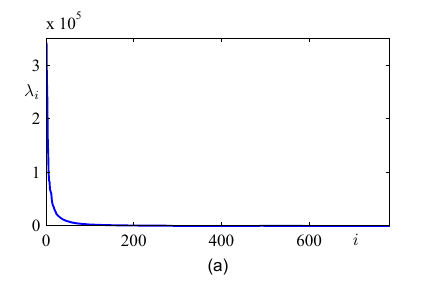
\includegraphics[scale = 0.7]{\figDir/eigenspectrum.PNG}
		\label{fig:eigenspectrum}
		\caption{Sorted eigenvalues plotted against index}
	\end{figure}
	\pagebreak
	In this case it seems like taking the top 50 eigenvectors to represent a reduced dataset would be a good approximation. An engineering rule would be to cut off at "the knee" where the eigenspectrum starts to plateau rapidly.

	\renewcommand{\this}{HMM_EM}

\chapter{Hidden Markov Models}

Talk about HMM use cases, sequential data, text processing, ... a bit outdated maybe.

\section{notation}
\begin{itemize}
\item $\mathcal{Z} = \{Z_1, ..., Z_T\}$: A random vector representing the categories, e.g. "verb".

\item $\mathcal{X} = \{X_1, ..., X_T\}$: A random vector representing the words, e.g. "work".

\item $\textbf{X}=\{x_1,...,x_T\}$: A \textbf{non-random} vector of \textbf{observations}, e.g a full scentence, note that $\textbf{X} \in O^T$.
		
\item $\textbf{Z}=\{z_1,...,z_T\}$: A \textbf{non-random} vector of \textbf{categories}, e.g a full scentence, note that $\textbf{Z} \in Q^T$.
		
\item $Q=\{q_1,...,q_K\}$: The collection of values $Z_i$ can take. Define $|Q|=K$.
		
\item $O=\{o_1,...,o_L\}$: The collection of words $X_i$ can take i.e. the corpus. Define $|O|=L$.

\item $A_{i\rightarrow j} = P(Z_t = q_j| Z_{t-1}=q_i)$: transition probability of going from category $i$ to category $j$. e.g. "Verb" $\to$ "Noun". Independent of $t$ since it's a markov chain.
		
\item $B_{i\rightarrow j} = P(X_t = o_j|Z_t = q_i)$: emission probability of emitting word $o_j$ if you're in category $i$. e.g. "Verb" $\to$ "work". Independent of $t$ since it's a markov chain.
		
\item $\theta$: collection of parameters $\theta = \{A_{ij,B_{ij}}, \pi\} \forall i,j$ here $\pi$ is the distribution of $Z_1$. i.e. Which "Adverb" is more likely as the category for the first word than "Verb".

\end{itemize}

Any hidden markov model can be represented as follows:
\begin{figure}[h!]
	\centering
	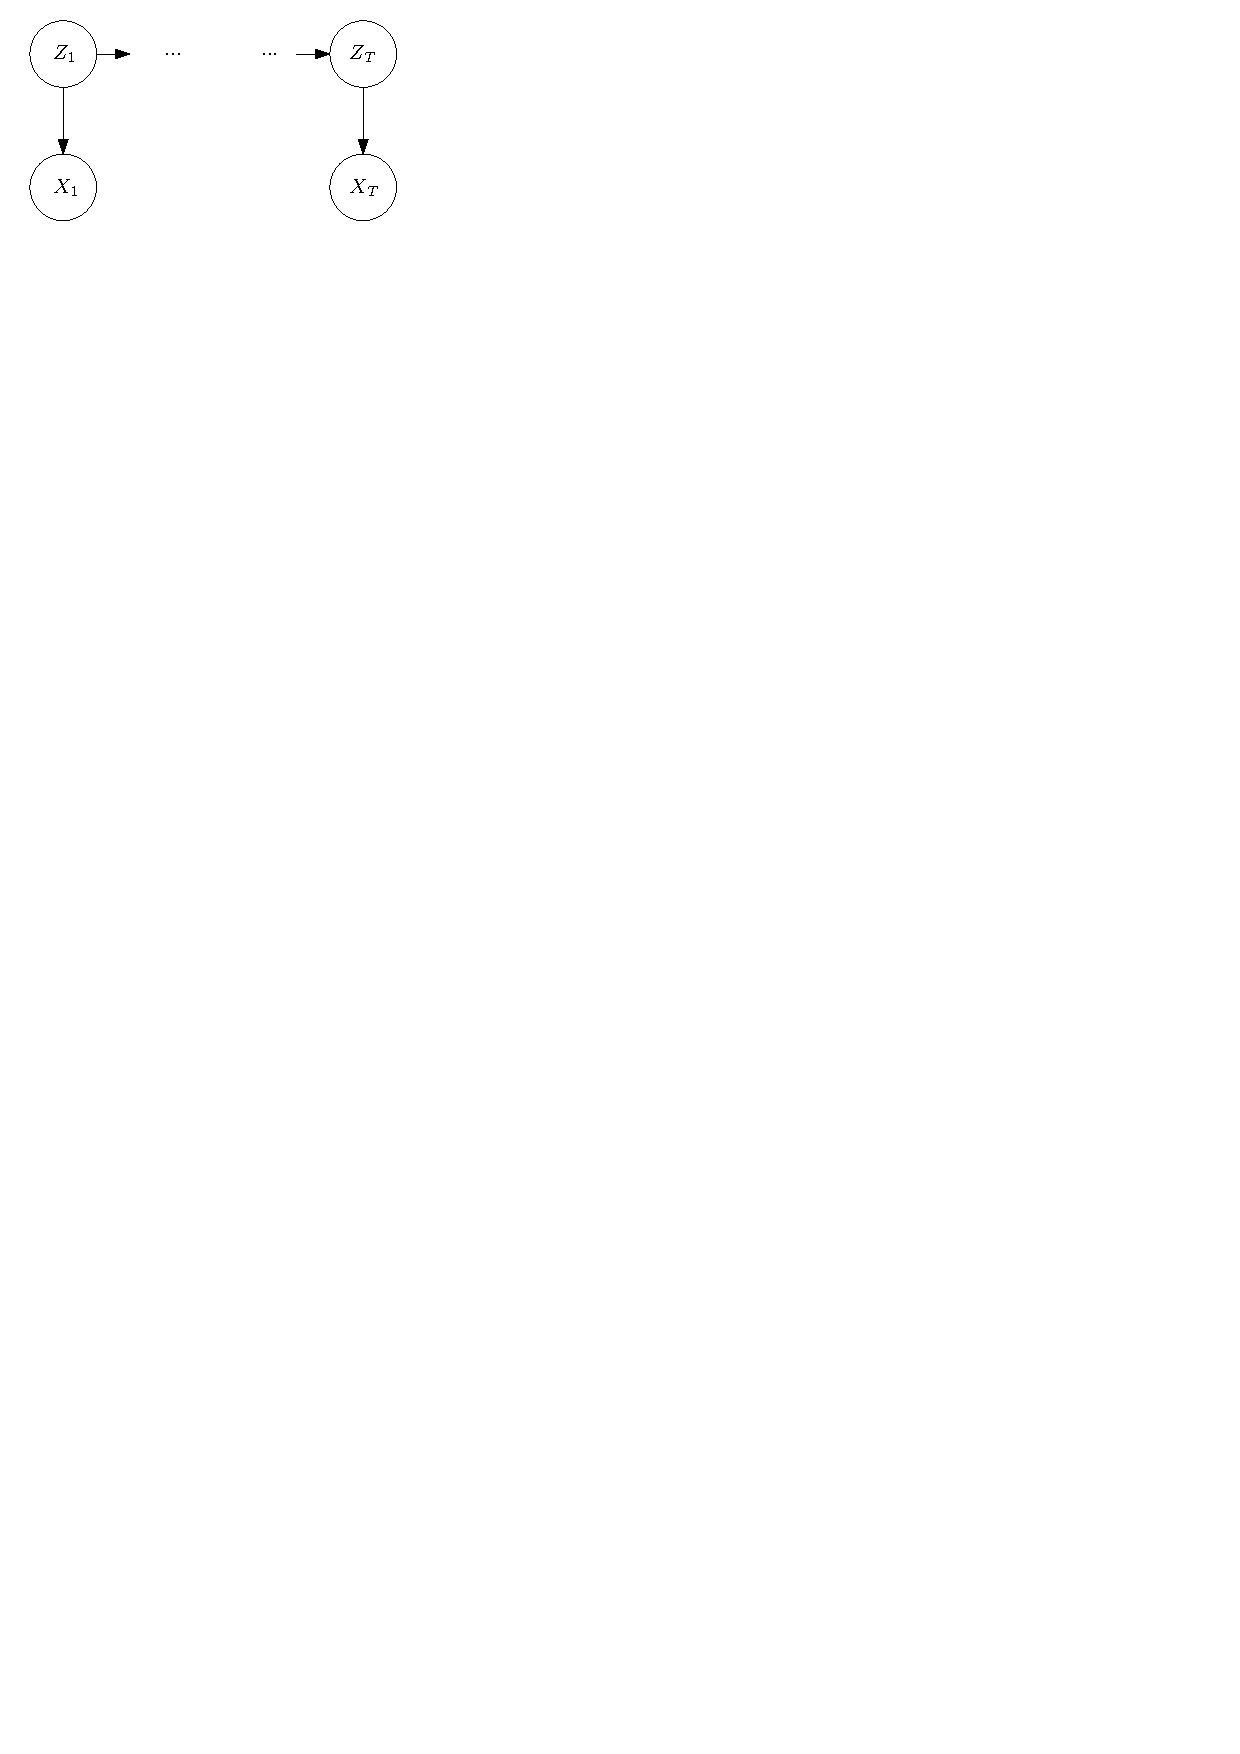
\includegraphics{\figDir/HMM.pdf}
\end{figure}
\section{Maximum likelihood for HMM}
\subsection{General principle of maximum likelihood}
	
Given data $\mathcal{X}$ that you assume comes from a probabilistic model $D \sim P(X|\theta)$. Maximum likelihood is a general principle in which you try to find parameters $\theta$ such that the data is "most likely" to occur. This means we find:

\begin{equation}
	\hat{\theta} = \underset{\theta}{\text{arg max }} P(D|\theta)
\end{equation}

However it is ofter easier to optimize the the $\log(.)$ of the likelihood function. Since $\log(.)$ is monotonically increasing minimizing this is by defninition identical, although often easier computationally.
\begin{equation}
	\hat{\theta} = \underset{\theta}{\text{arg max }} P(D|\theta) = \underset{\theta}{\text{arg max }} \log(P(D|\theta))
\end{equation}
	
I will denote the log liklihood as $L(D|\theta)$.\\\\

\textbf{Example:} Intuitively if we flip a coin 100 times and find 20 heads(=0) and 80(=1) tails. The parameter of this Bernouilli variable will more likely be higher than $p=0.5$.
	
\subsection{MLE for HMM}
\subsubsection{Likelihood of HMM}
Likelihood of a Hidden Markov Model is found by "pluggin in" bayesian network:
\begin{equation}
	\begin{split}
	P(\mathcal{Z},\mathcal{X}|\theta) &= \prod_{t=0}^{T-1}\underbrace{P(Z_{t+1}|Z_t)}_{transition}\underbrace{P(X_{t+1}|Z_{t+1})}_{emission}
	\end{split}
\end{equation}

Where $P(Z_1|Z_0) = P(Z_1)$, is the prior of the bayes net.
For hidden markov models we have addictional constraints on the parameters namely:
\begin{equation}
	\begin{split}
	\sum_{j=1}^{K}p(Z_{t+1} = q_j|Z_t = q_i)=\sum_{j=1}^{K} A_{i\rightarrow j} &= 1 \indent \forall i\\
	\sum_{j=1}^{L}p(X_{t} = o_j|Z_t = q_i)=\sum_{j=1}^{L} B_{i\rightarrow j} &= 1 \indent \forall i
	\end{split}
\end{equation}
	
Meaning that for every category in our set $Q$ the total probability of going to any state is 1 and the total probability of seeing any word should be 1.
	
\subsubsection{Small comment}
For HMM we can try to apply the maximum likelihood estimate. Since the likelihood for a HMM is given in terms of the observations $\textbf{X}=\{x_1,...,x_T\}$ and the known categories $\textbf{Z}=\{z_1,...,z_T\}$, in order to perform maximum likelihood we need both of these. This would for example mean that someone would categorise every word in a book before estimating the parameters, which some might consider impossible. However for now we assume this is no problem and continue.
	
\subsubsection{Actual calculation}
Almost all ML methods we will be maximizing the log-likelihood instead, note that in the following we no longer assume no data but instead assume observations $\textbf{X}$ and categories for these $\textbf{Z}$:
\begin{equation}
	\begin{split}
	\hat{\theta} = &\underset{A,B,\pi}{\text{arg max }}\log(\prod_{t=0}^{T-1}P(Z_{t+1} = z_{t+1}|Z_t=z_t)P(X_{t+1}=x_{t+1}|Z_{t+1}=z_{t+1}))\\
	&= \underset{A,B,\pi}{\text{arg max }} \sum_{t=0}^{T-1} log(P(Z_{t+1} = z_{t+1}|Z_t=z_t)) + \sum_{t=0}^{T-1} \log(P(X_{t+1}=x_{t+1}|Z_{t+1}=z_{t+1}))\\
	&=\underset{A,B,\pi}{\text{arg max }} \sum_{t=0}^{T-1} log(A_{t\rightarrow t+1}) + \sum_{t=0}^{T-1} \log(B_{t\rightarrow t})\\
	\end{split}		
\end{equation}
	
Note the notation it quite confusing at this point, however $A_{t\rightarrow t+1}$ is the probability of going from \textbf{observed} category at step $t$ in the chain to what we \textbf{observed} in step $t+1$. Same goes for $B_{t\rightarrow t}$.\\\\
So what's next? We know the parameters are optimal if the gradient w.r.t. the parameters is 0, i.e. $\nabla L(\textbf{X},\textbf{Z}|\theta) = 0$. However if we do this we overlooked a key component which are the extra constraints we placed on the parameters. A quick look at whet we maximize shows us that setting all parameters to $\infty$ is optimal, however clearly doesn't result in a proper transition or emission distribution. To include the constraints we use lagrange multipliers\footnote{Look at wikipedia for a quick guide, a really usefull trick to know in any field that uses any form of optimization: \url{https:// en.wikipedia.org/wiki/Lagrange_multiplier}}:
\begin{equation}
	\mathcal{L}(\theta, \lambda, \alpha) = \sum_{t=0}^{T-1} log(A_{t\rightarrow t+1}) + \sum_{t=0}^{T-1} \log(B_{t\rightarrow t})\\
	+\sum_{i}^{K}\lambda_i(1-\sum_{j}^{K}A_{i\rightarrow j}) +\sum_{i}^{K}\alpha_i(1-\sum_{j}^{L}B_{i \rightarrow j})
\end{equation}
The above function is called the lagrangian. Now all we have to do is optimize this. Since the general lagrange theory says that for optimal solution $\hat{\theta}$ of the constrained problem, there exists $\hat{\lambda}$ and $\hat{\alpha}$ such that $(\hat{\theta},\hat{\lambda}, \hat{\alpha})$ is a stationary point of $\mathcal{L}(\theta, \lambda, \alpha)$. In short, we can maximize $\mathcal{L}(\theta, \lambda, \alpha)$ and find $\lambda$ and $\alpha$ instead of doing constrained optimization. First we find the the optimal transtion parameters, the emission parameters are identical by symmetry of the lagrangian.
\begin{equation}
		\begin{split}		
		\frac{\partial}{\partial A_{f\rightarrow s}}\mathcal{L}(\theta, \lambda, \alpha) =& \frac{\partial}{\partial A_{f\rightarrow s}}\left(\sum_{t=0}^{T-1} log(A_{t\rightarrow t+1})\right) + \sum_{t=0}^{T-1}0 + \frac{\partial}{\partial A_{f\rightarrow s}}\left( \sum_{i}^{K}\lambda_i(1-\sum_{j}^{K}A_{i\rightarrow j})\right)+\sum_{i=0}^{K}0\\
		=&  \left(\sum_{t=0}^{T-1} \frac{\mathbbm{1}[x = A_{f\rightarrow s}](A_{t\rightarrow t+1})}{A_{f\rightarrow s}}\right) - \lambda_{f}
		\end{split}
\end{equation}

To derive the lagrangian we see that the components which do not contain $A_{f\rightarrow s}$ derive to $0$. In the first sum only the observations of $A_{f\rightarrow s}$, i.e. when we observe going from category $f$ to $s$., will derive to $\frac{\partial}{\partial A_{fs}} \log A_{f\rightarrow s} = \frac{1}{A_{f\rightarrow s}}$. Hence the indicator function $\mathbbm{1}[x = A_{f\rightarrow s}](A_{t\rightarrow t+1})$, it is $0$ when the input $A_{t\rightarrow t+1}$ is not $A_{f\rightarrow s}$. Now setting the derivative to zero to find optimality:

\begin{equation}
	\begin{split}
	\left(\sum_{t=0}^{T-1} \frac{\mathbbm{1}[x = A_{f\rightarrow s}](A_{t\rightarrow t+1})}{A_{f\rightarrow s}}\right) - \lambda_{f} &= 0\\
	\frac{count(f\rightarrow s)}{A_{f\rightarrow s}} &= \lambda_f\\
	A_{f\rightarrow s} &= \frac{count({f\rightarrow s})}{\lambda_{f}}
	\end{split}
\end{equation}
	
However now we need to find what $\lambda_f$ is. We do this by enforcing the transition constraint, that is from any category $f$ we must go to any other state $s$. In formula we want $\sum_{j=1}^{K} A_{i\rightarrow j} = 1 \indent \forall i$:
\begin{equation}
	\begin{split}
	\sum_{j=1}^{K} A_{i\rightarrow j} &= 1\\
	\sum_{j=1}^{K} \frac{count({f\rightarrow j})}{\lambda_{f}} &= 1\\
	\sum_{j=1}^{K} count({f\rightarrow j}) &= \lambda_f
	\end{split}
\end{equation}
	
We find $\lambda_f$ to be the total amount of time a transition starting in $f$ is observed. We find the estimate of $A_{fs}$ simply as the fraction:

\begin{equation}
	\hat{A}_{f\rightarrow s} = \frac{count({f\rightarrow s})}{\sum_{j=1}^{K} count({f\rightarrow j})}
\end{equation}
	
The fraction of times you observe a transition from $f$ to $s$ compared to the total amount of times a transition from $f$ to any state is observed.
\\\\
Note by looking at the lagrangian we find symmetry and the maximum likelihood estimate of $B_{fo}$ can be derived in exactly the same way as the maximum likelihood for $A_{fs}$, resulting in:

\begin{equation}
	\hat{B}_{fo} = \frac{count({f\rightarrow o})}{\sum_{o=1}^{L}count({f\rightarrow o})}
\end{equation}

Again the notation doesn't work out very nice, however it explains the situation. Again the maximum likelihood estimate for observing word $o$ given category $f$ is the fraction of times we observe $o$ in category $f$ compared to the amount of times we observe category $f$. Note a special case is $A_{0j}$ which is then simply the fraction of times we observe category $j$ compared to the rest of the categories.

\section{EM for HMM}
Expectation maximization is a general and widely used algorithm in machine learning to deal with either missing data or unobserved/latent variables to maximize the parameters of a model. It does this by estimating the likelihood iteratively and adapting the parameters.

\subsection{EM in \textbf{general}}
This part is based on the wikipedia article on EM\footnote{\url{https://en.wikipedia.org/wiki/Expectation_maximization_algorithm}}. Note that I use the same notation of the wikipedia article, $\textbf{Z}$ does not denote categories in a HMM nor does $\textbf{X}$ represent observations. In fact in the following we don't even assume that our model is a HMM.
Say we have a statistical model that generates $\textbf{X}$ observed data and $\textbf{Z}$ unobserved data. This model is parameterized by \textbf{$\theta$}, then the likelihood of this observed/unobserved data is defined as:
\begin{equation}
\begin{split}
L(\theta;\textbf{X}) &= \sum_{z} L(\theta;\textbf{X},z)\\
&= \int_{Z}L(\theta;\textbf{X},z)dz
\end{split}
\end{equation}
We could try to maximize this quantity over $\theta$, and this would work perfectly fine. However, this often proves intractable since we have to sum/integrate over $Z$.\\

Since this is intractable, in practice the EM algorithm is used instead. The EM algorithm consists of the following 2 steps:
\begin{equation}
Q(\theta|\theta^{(t)}) = \mathbb{E}_{\textbf{Z}|\textbf{X}, \theta^{(t)}}[\log L(\theta;\textbf{X},\textbf{Z})]
\end{equation}
Which is the expectation over $\textbf{Z}$ given observed data $\textbf{X}$ and previous $\theta^{(t)}$ of the log-likelihood of observed and unobserved data. This is called the \textbf{Expectation} step.
\begin{equation}
\theta^{(t+1)} = \underset{\theta}{\text{arg max }} Q(\theta|\theta^{(t)}) 
\end{equation}
The update for $\theta^{(t)}$ is the maximization of $Q$. This is called the \textbf{Maximization} step.
\pagebreak
\subsection{EM for HMM}
We can apply EM for HMM, in previous section I tried to emphasise the fact that $\textbf{Z}$ just denoted variables we don't know or are latent and not specifically the categories of a HMM. However in the case of HMM $\mathcal{Z}$ actually are the latent variables. Aswell as $\mathcal{X}$ being the observed variables.
\subsubsection{Expectation in HMM}
Plugging in the definition using the log liklihood of HMM and the definition of expectation for discrete variables we find:
\begin{equation}
\begin{split}
\mathbb{E}_{\textbf{Z}|\textbf{X}, \theta^{(t)}}[\log L(\theta;\textbf{X},\textbf{Z})] &= \sum_{\textbf{Z}}p(\textbf{Z}|\textbf{X},\theta^{(t)})\left(\sum_{t=0}^{T-1} log(A_{t,t+1}) + \sum_{t=0}^{T-1} \log(B_{tt}) \right)\\
=& \sum_{\textbf{Z}}p(\mathbf{Z}|\mathbf{X},\theta^{}(t))log(A_{0,1}) + ... + \sum_{\textbf{Z}}p(\mathbf{Z}|\mathbf{X},\theta^{}(t))log(A_{T-1,T}) \\&+ \sum_{\textbf{Z}}p(\mathbf{Z}|\mathbf{X},\theta^{}(t))log(B_{11})\\
\end{split}
\end{equation}
Note thet we are summing over $\textbf{Z}$, this is the vector of categories in each timestep. More formally we can actually write:
\begin{equation}
\sum_{\textbf{Z}} = \sum_{z_1}\sum_{z_2}...\sum_{z_T}
\end{equation}
In order to make life easier we look at what happens to a single term of the form $log(A_{t,t+1})$ by taking the sum inside, more concretely what I mean is the following:
\begin{equation}
\begin{split}
\sum_{z_1}\sum_{z_2}...\sum_{z_T}p(z_1,...,z_T|\mathbf{X},\theta^{(t)})log(A_{i,i+1})
\end{split}
\end{equation}
\end{document} 

	
\end{document}